\section{Durchführung}
\label{sec:Durchführung}

\subsection{Messung bis 1 bar}
Die in Abbildung \ref{fig:aufbau1} dargestellte Apparatur wird aufgebaut. Zu Anfang wird sie mittels einer Wasserstrahlpumpe evakuiert.
Dafür wird das Drosselventil und der Absperrhahn geöffnet und das Belüftungsventil geschlossen. Nachdem sich ein für das Experiment akzeptabler Druck eingestellt hat, wird das
Drosselventil und der Absperrhahn geschlossen und die Wasserstrahlpumpe ausgestellt. Anschließend wird die Heizhaube eingeschaltet, so dass sich die Flüssigkeit erhitzt. Um 
aufsteigenden Dampf zu kondensieren wird zusätzlich die Kühlung angestellt. Die Temperatur wird durch ein Thermometer bestimmt, das sich im Mehrhalskolben befindet und der Druck
wird am Manometer abgelesen. Der Druck und die Temperatur werden paarweise gemessen bis 1 bar erreicht wird.
\begin{figure}
    \centering
    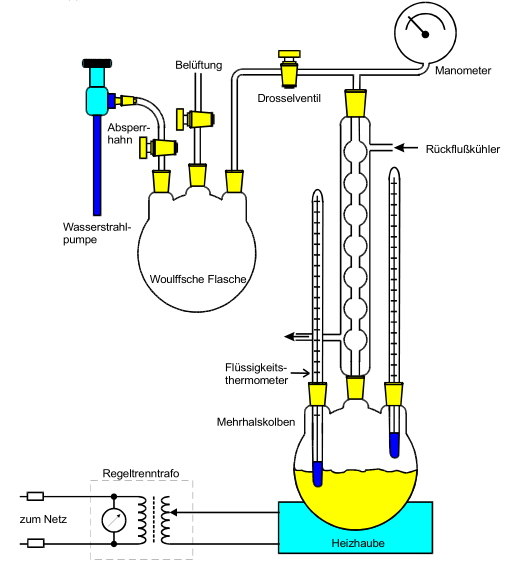
\includegraphics{Aufbau1.png}
    \caption{Aufbau 1 \cite{sample}}
    \label{fig:aufbau1}
\end{figure}

\subsection{Messung von 1 bis 15 bar}
Die verwendete Apparatur ist in Abbildung \ref{fig:aufbau2} dargestellt. Vor Beginn des Versuchs ist schon Wasser in der Schale, so dass nur noch die Heizung eingeschaltet
werden muss. Dann werden in 1 bar Schritten die Messwerte aufgenommen.
\begin{figure}
  \centering
  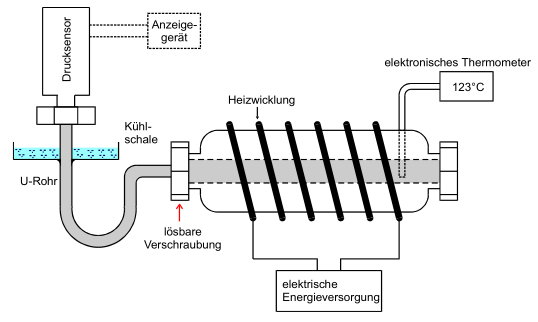
\includegraphics{Aufbau2.png}
  \caption{Aufbau 2 \cite{sample}}
  \label{fig:aufbau2}
\end{figure}